% TALK ABOUT HYDRA AND HOW THE ORGANISMS CAN REGENERATE PARTS OF ITS BODY.

\section{Hydra Morphogenesis and regenerative properties}

\subsection{Anatomy of a Hydra}

Hydras are fascinating organisms. Despite their rather small size (roughly 5mm of length in average), they are capable of extraordinary regenerative properties that allows them to fully reconstruct their body out of a very small portion of tissue (see figure \ref{hydraregen}).
\begin{figure}
\label{hydraregen}
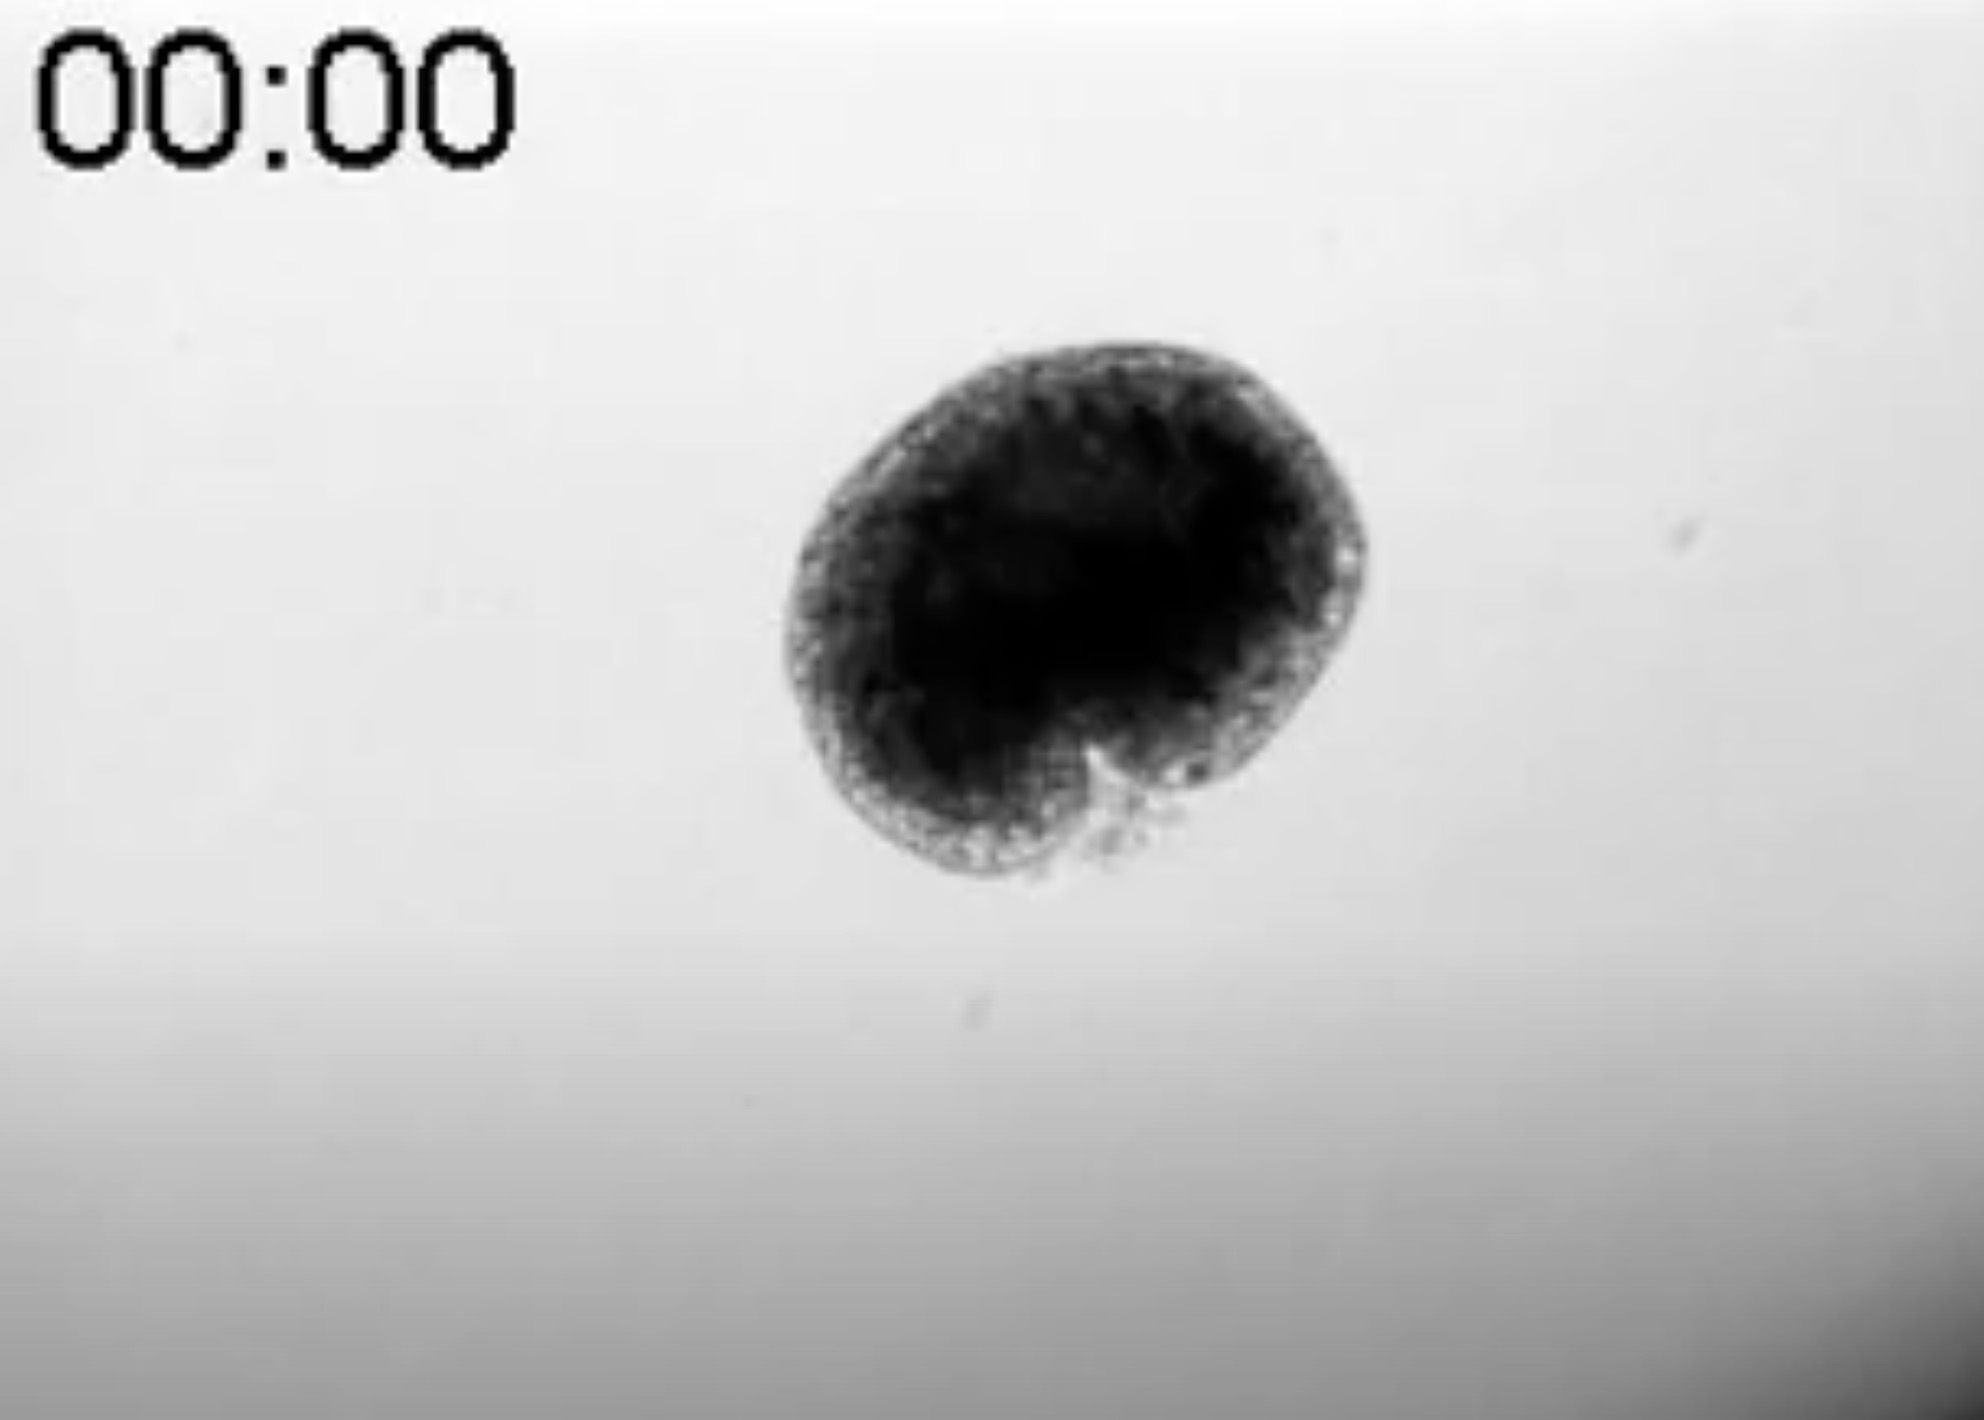
\includegraphics[width=0.19\textwidth]{figures/hydra_growth1}
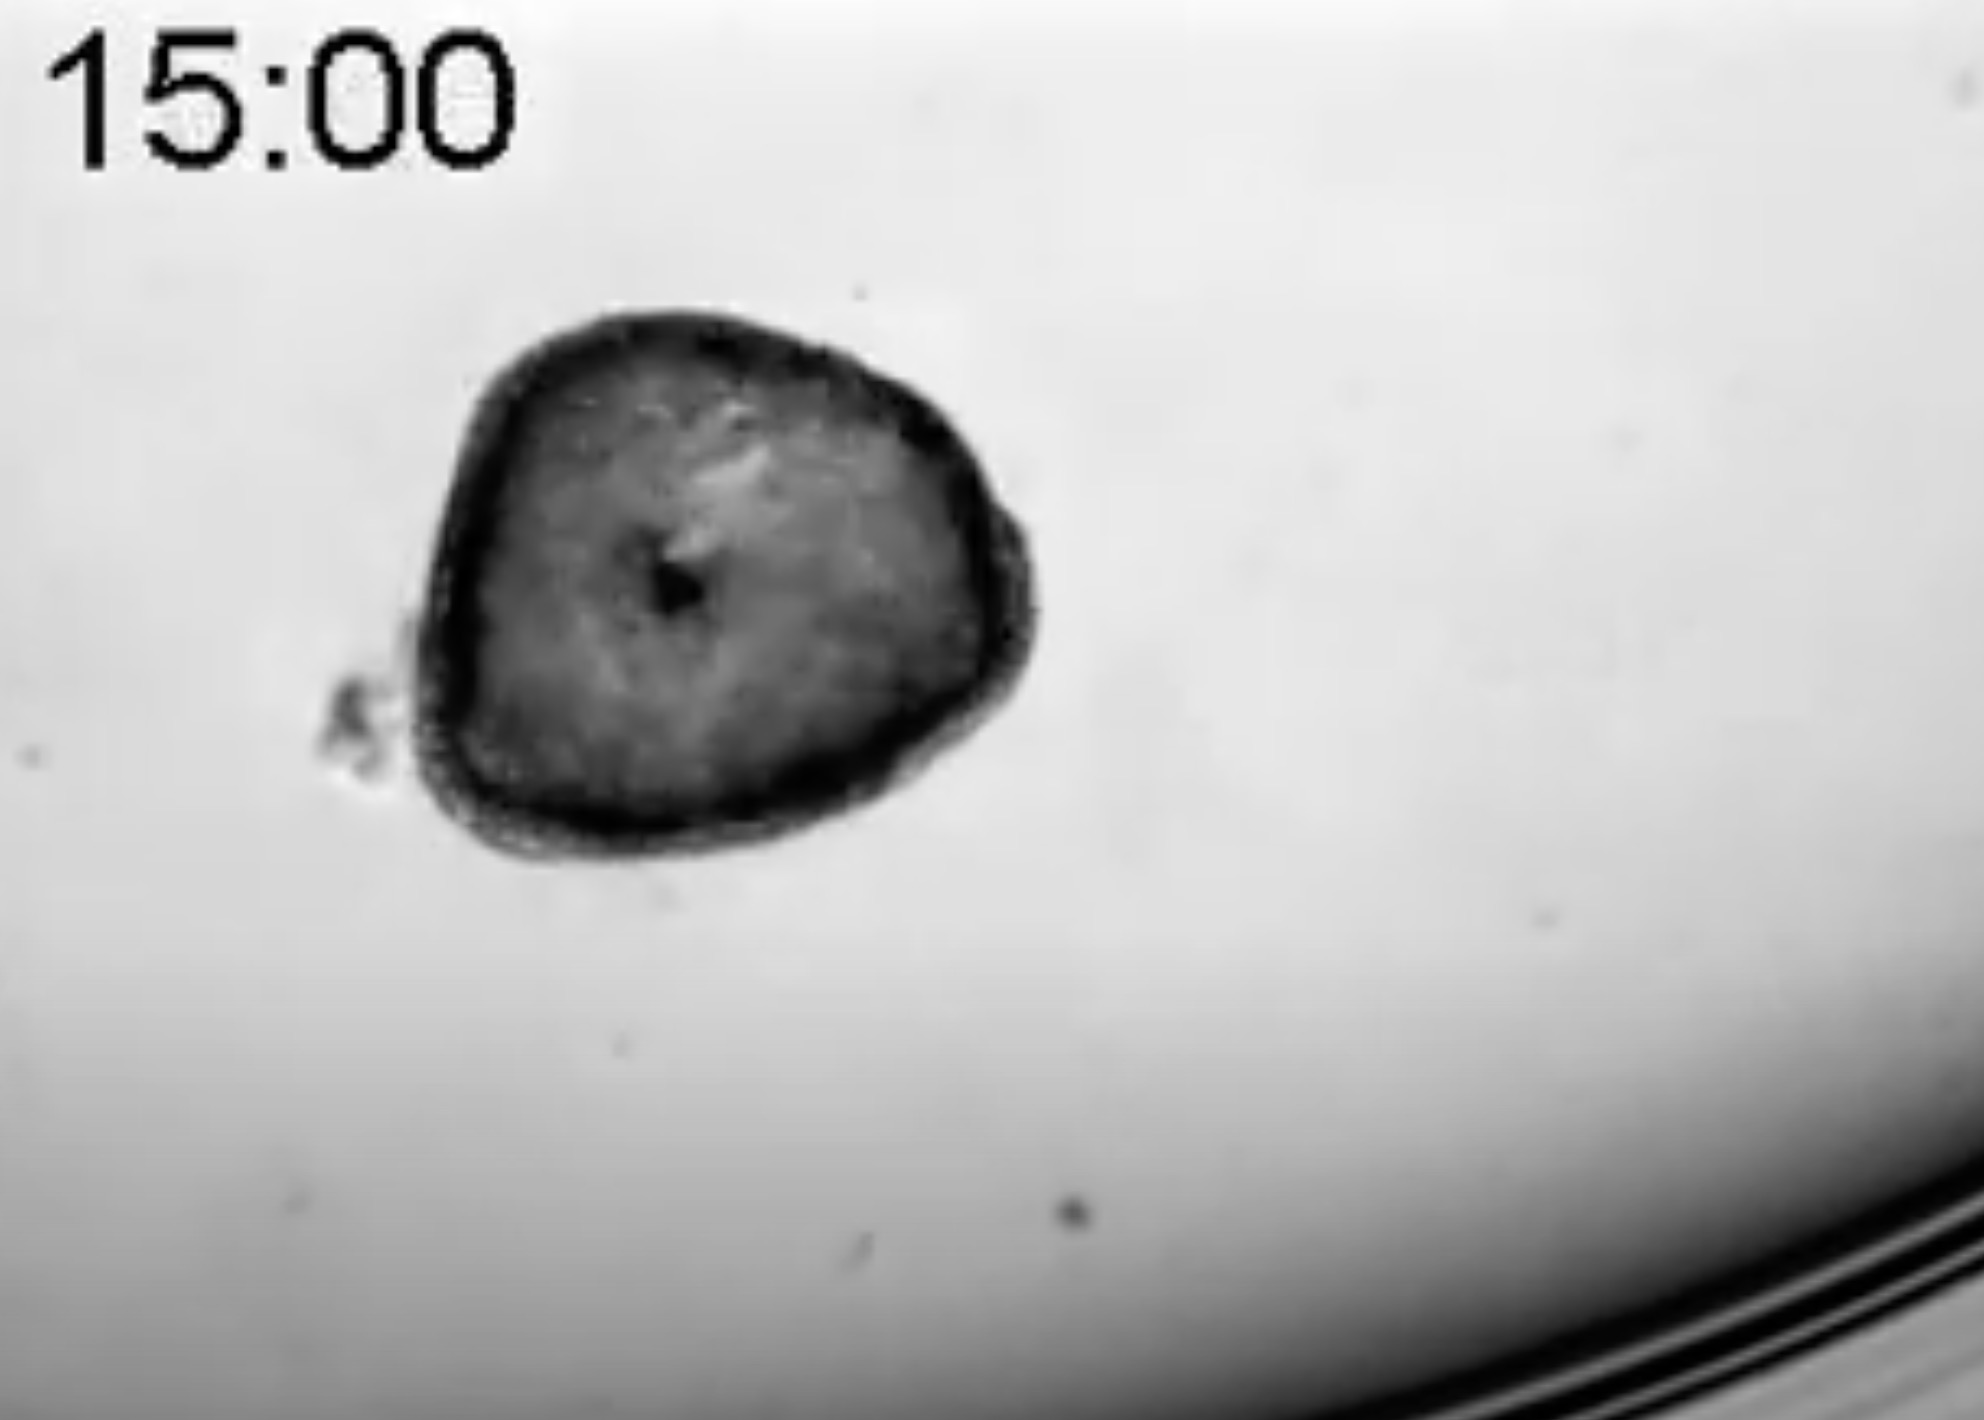
\includegraphics[width=0.19\textwidth]{figures/hydra_growth2}
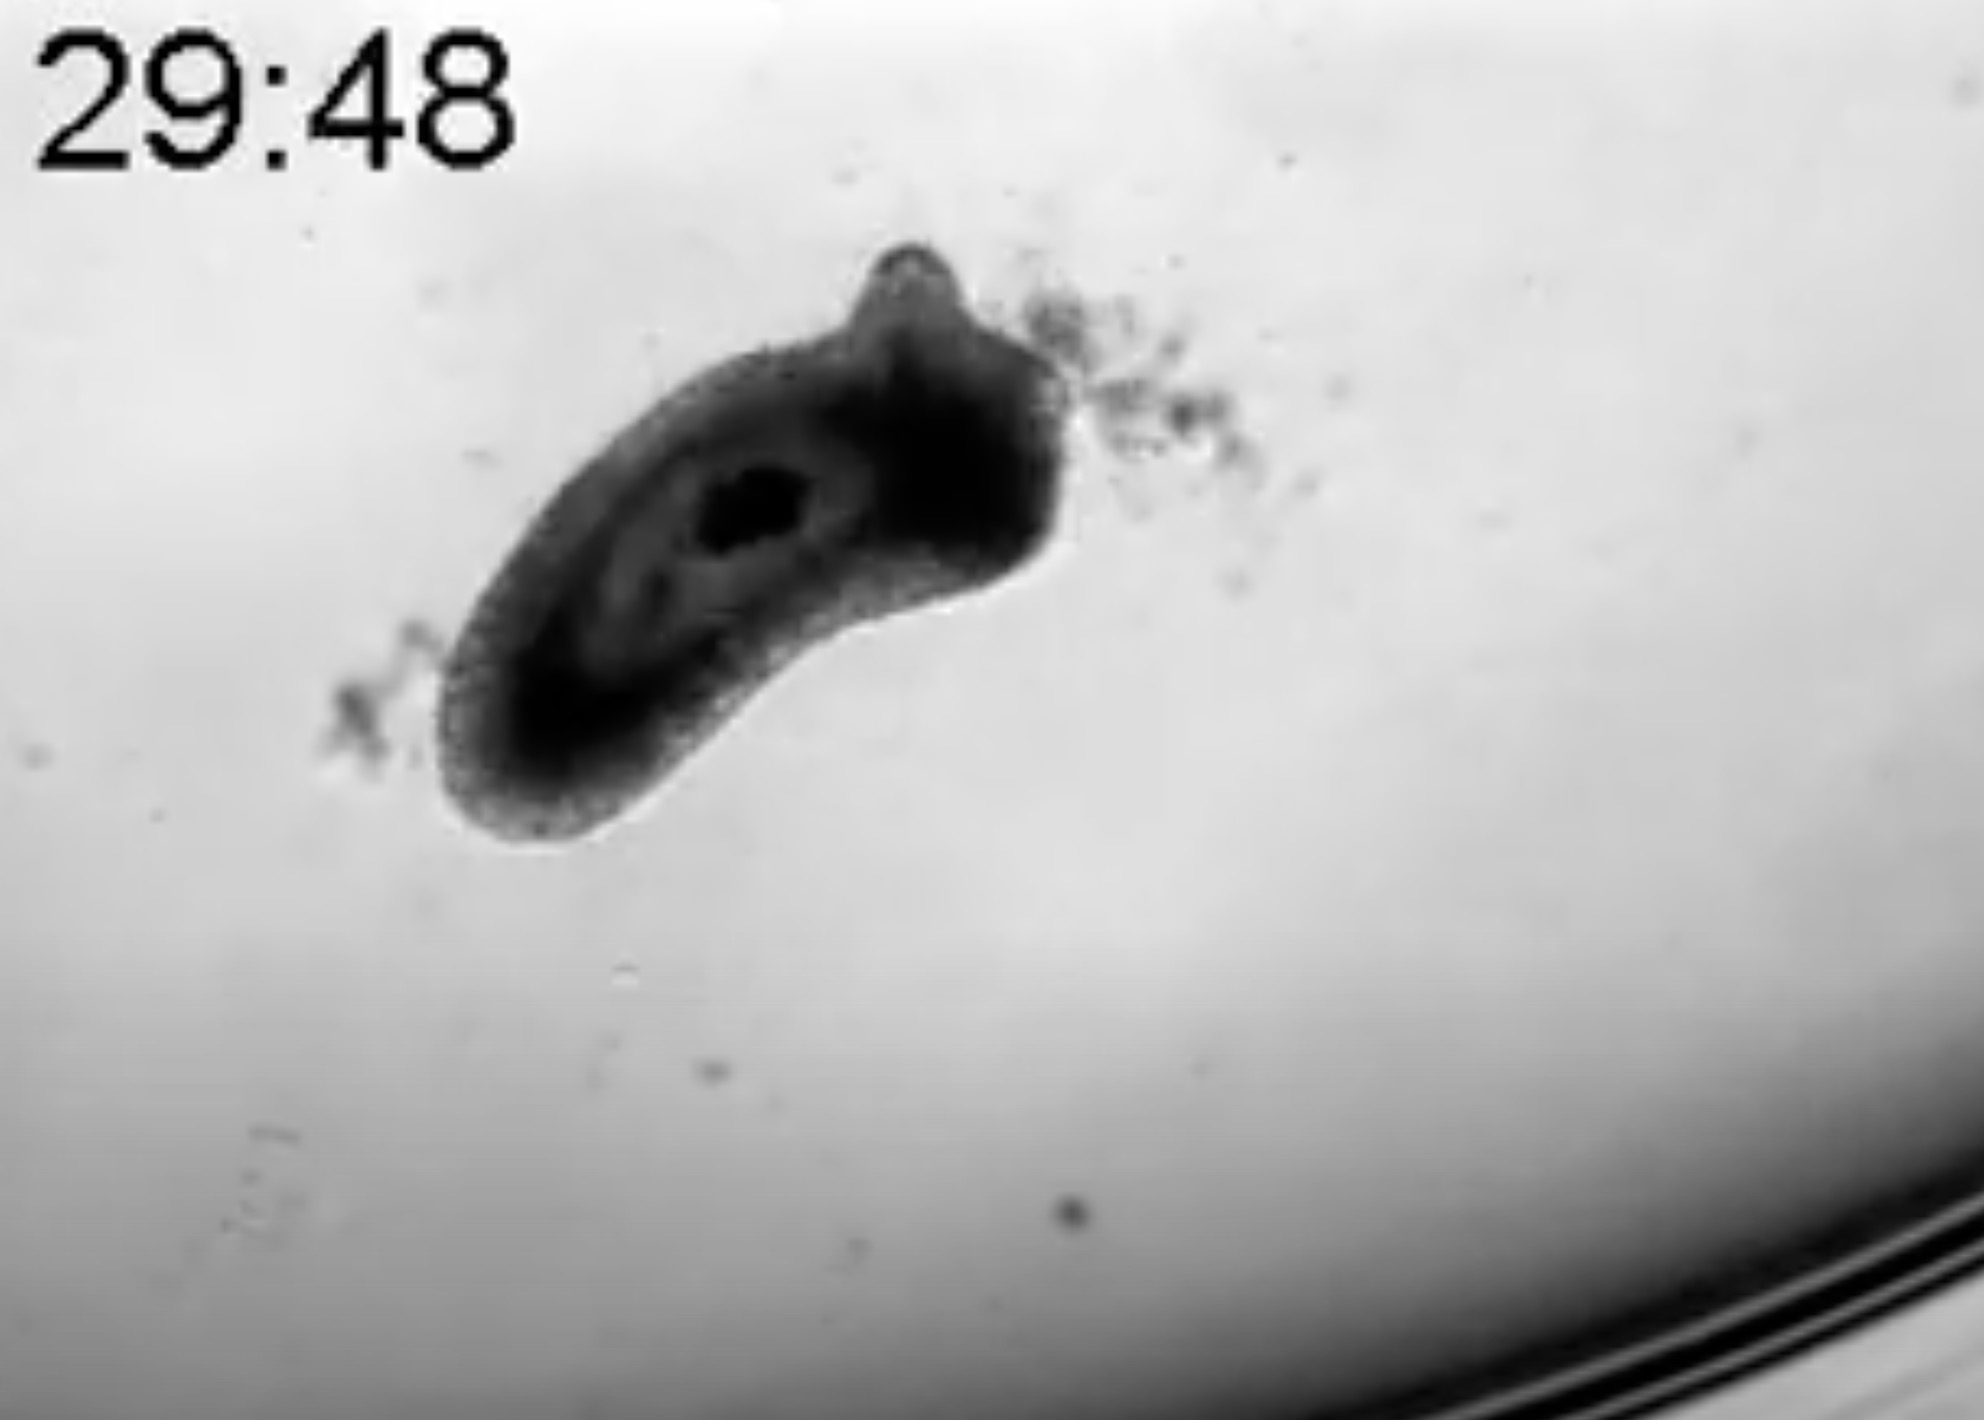
\includegraphics[width=0.19\textwidth]{figures/hydra_growth3}	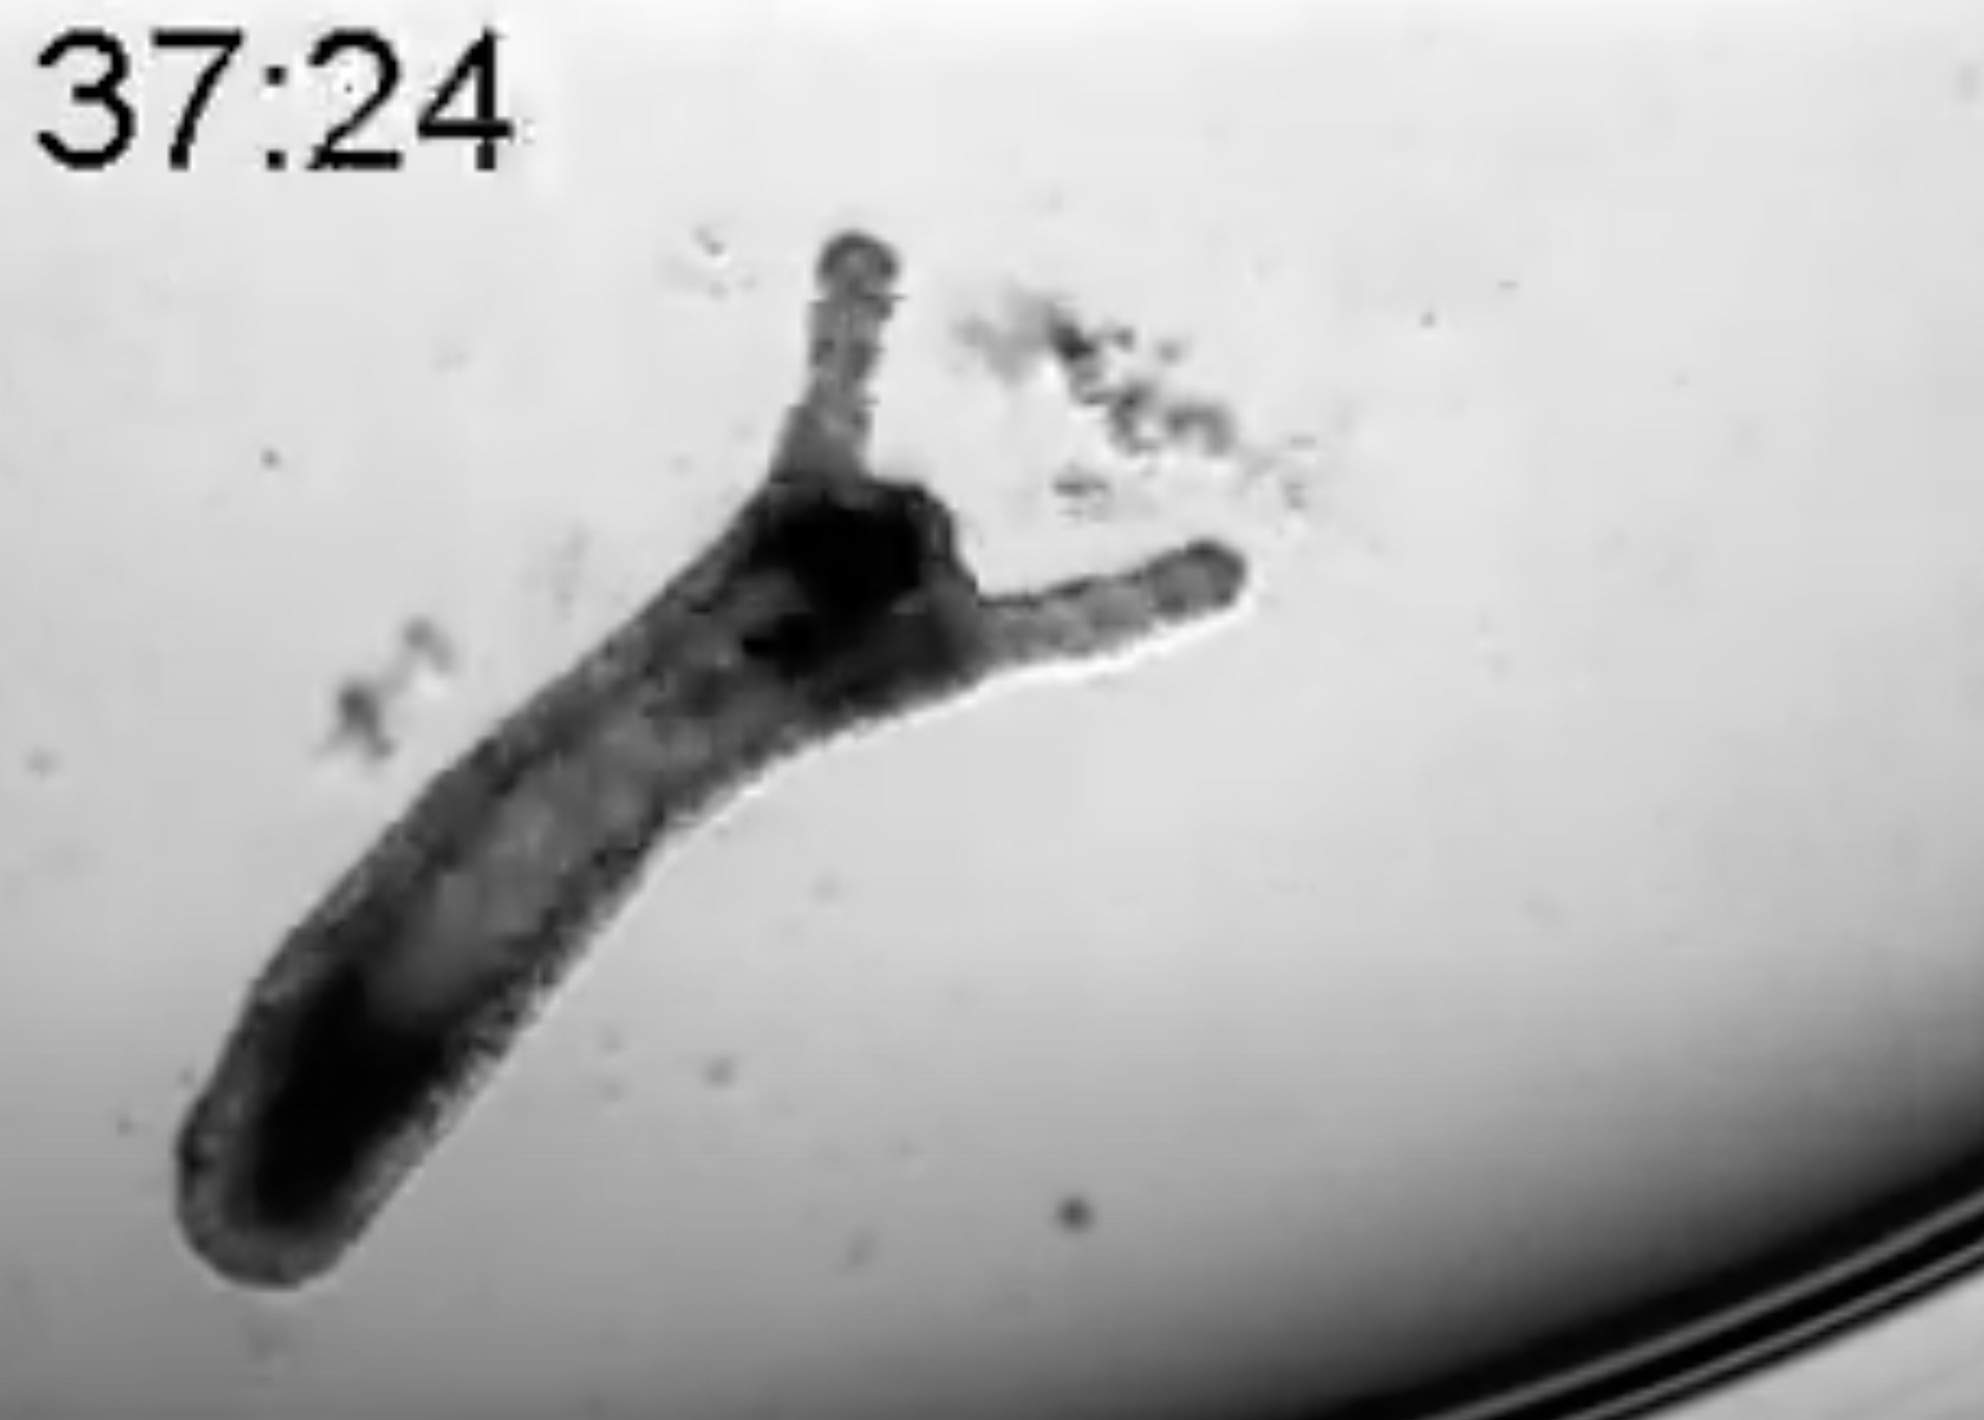
\includegraphics[width=0.19\textwidth]{figures/hydra_growth4}
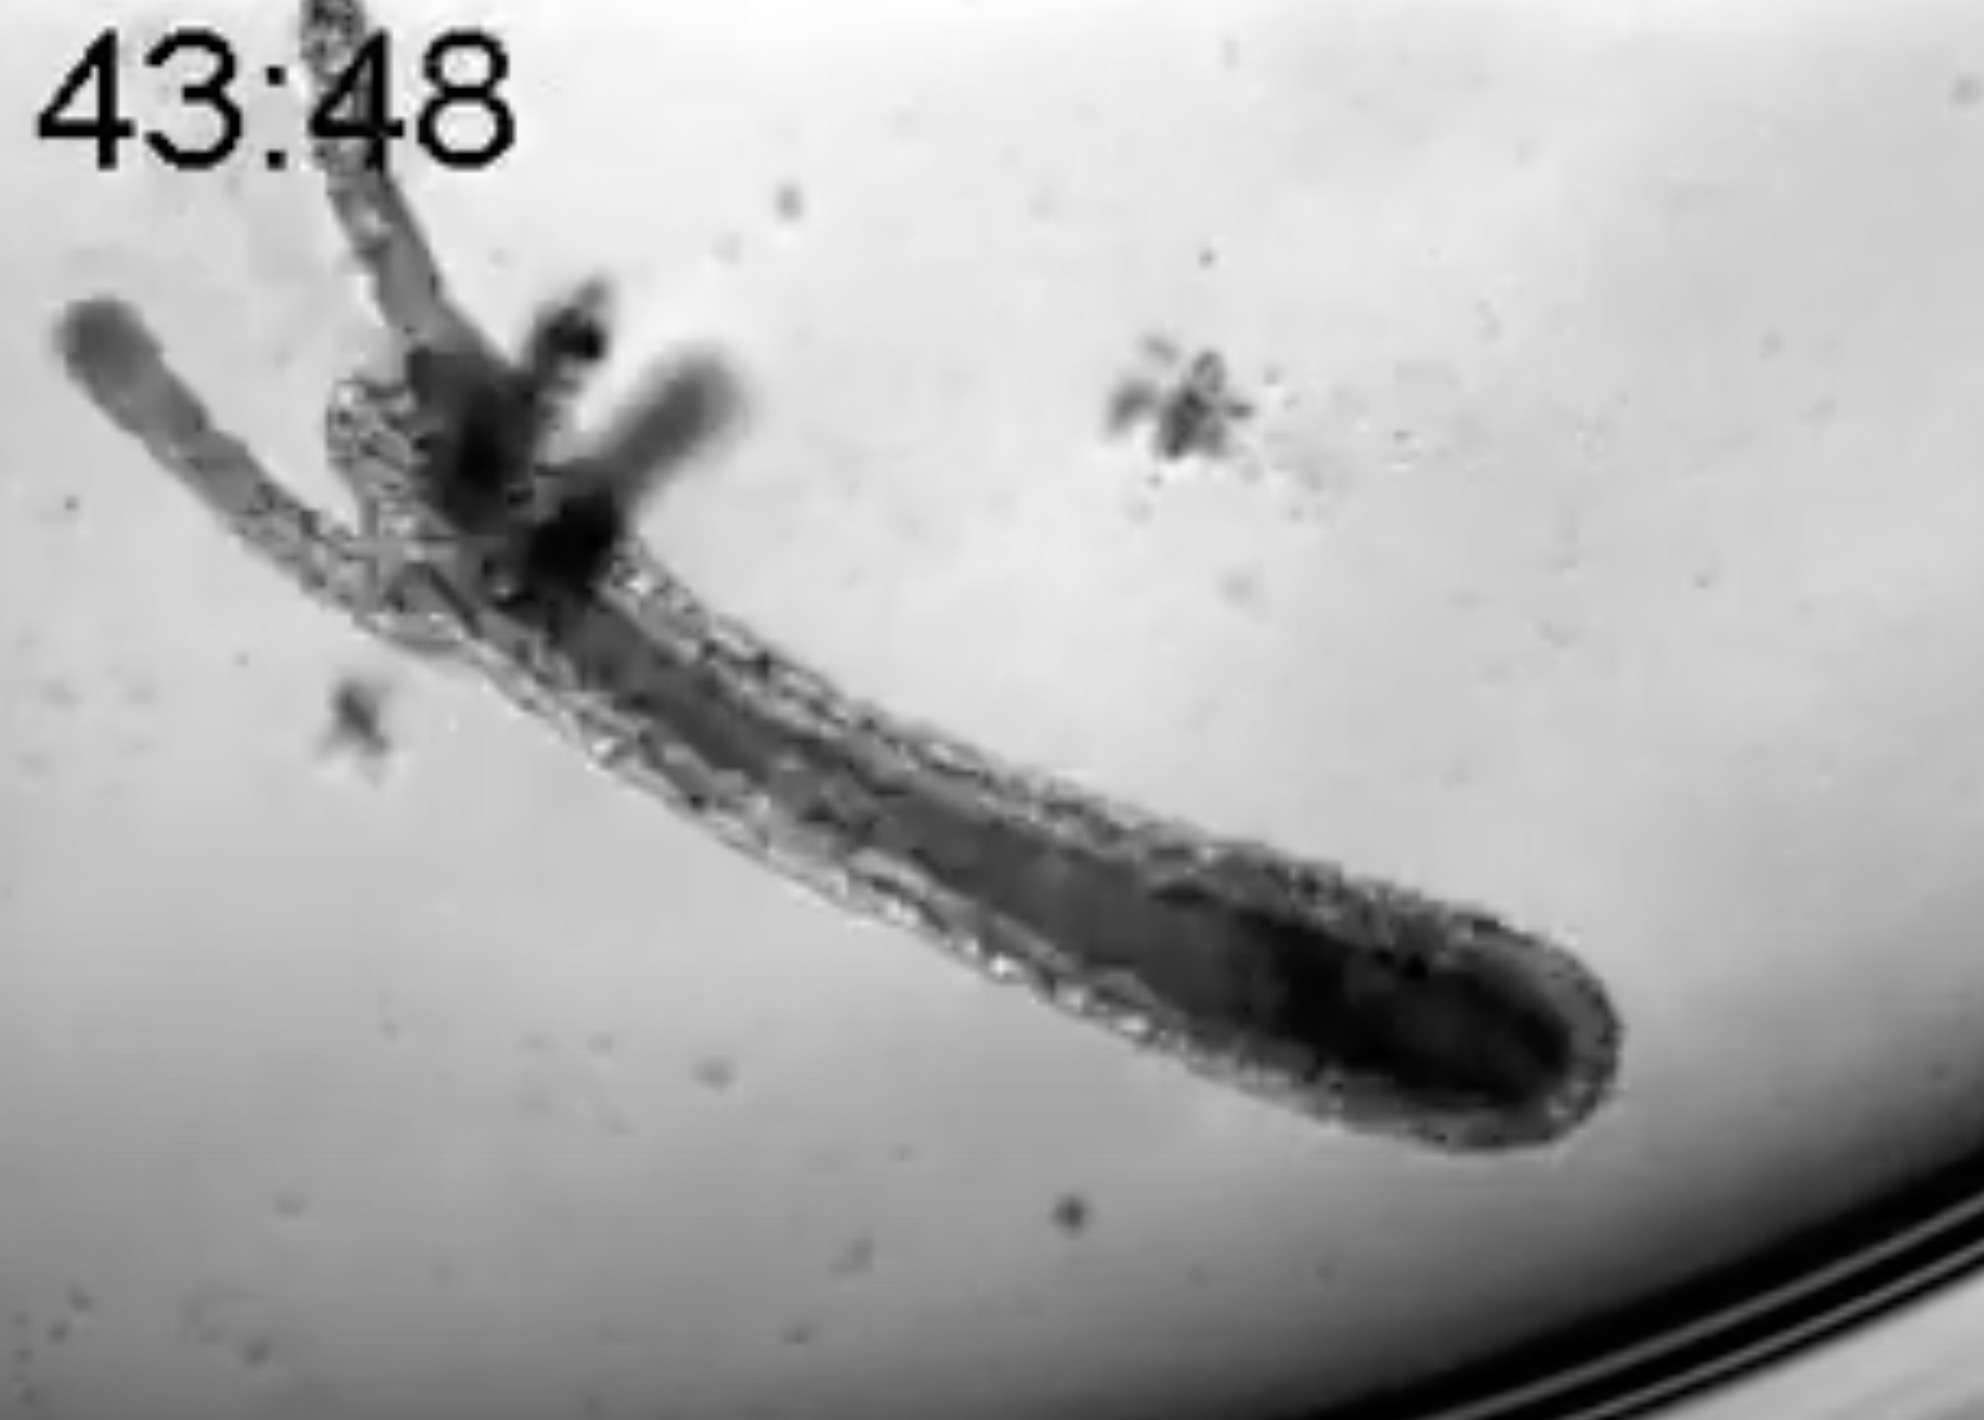
\includegraphics[width=0.19\textwidth]{figures/hydra_growth5}
\caption{Sequence of pictures taken under a traditional microscope. It shows how a Hydra is capable of regenerating its entire body from a small extracted sample of tissue coming from the body column (tissue diameter about 100 $\mu$m) of another Hydra. The timestamp on each picture is formatted as "hours:minutes", meaning the entire regeneration process takes place within the span of two days only.}
\end{figure}

Their body is composed of essentially three regions: the head, body column and foot. Spatially speaking, the small cnidarian is symmetrically organized around the oral-aboral axis giving it its hollow, tubular shape. Taking a step closer on each parts, one can notice that the head is composed of two sub-regions, one being a set of tentacles while the other one is called hypostome and acts as a mouth (it is also the only orifice in the whole organism). The foot, on the other hand is composed of a basal disc that allows hydras to stick to leaves and rocks - among others - underwater. Lastly, the body column is a long hollow tube made of cells undergoing constant mitosis through the life of the polyp. This ensures a constant cellular turnover of the derm (+ add why is it good). 

\subsection{Hydra reproduction and selection}

The way Hydras reproduce is very beneficial to the scientific community since they are able to reproduce either sexually or asexually (with the second one being the most common way of reproduction). The main difference between these two methods is that asexual reproduction preserves the totality of information in one individual, letting one the ability to "keep" a specific Hydra with nice genetic information for further reproduction. It is possible to repeatedly multiply a specific organism through asexual reproduction yielding   

\subsection{The importance of Wnt signaling}

\section{Emergence of Patterns and Diffusion-Driven Instability}
How do patterns form? Pattern formation is the result of the collaboration of a large amount of biological processes ranging from the nanoscopic up to the microscopic scale. Together, they form motifs, which we define as the structural organization of cells in space and time, often leading to pretty shapes such as the fur coat in animals or that on the wings of a butterfly. In his pioneer paper  published in 1952 [\bref{ref}], Alan Turing proposes a chemical model for pattern formation involving two chemical species: one Activator ($u$), one Inhibitor ($v$) \incl{(Probably inspired from the Lotka-Volterra prey-predator model introduced in 1910 which was itself applied to mathematical biology for the first time in 1926)}. The concentration of each specie is described with 2-morphogens reaction-diffusion equations with appropriate boundary conditions, \textit{i.e.} equations of the form 


\begin{align}
	\del_t u &= d_1 \lap u + f(u, v) &\text{on} \ \R^{+} \times \Omega \notag \\[0.7em]
	\del_t v &= d_2 \lap v + g(u, v) & \text{on} \ \R^{+} \times \Omega \\[0.7em]
	\del_\nu u & = 0; \quad \del_\nu v = 0 & \text{on} \ \del\Omega \notag \\[0.7em]
	u(0, x) &= u_0(x) ; \quad v(0, x) = v_0(x) & u_0, v_0 \in X
\end{align}
\label{eq:TuringModel}


for a specific choice of $f$ and $g$ describing the chemical kinetics of the reaction. This choice is usually what determines the model type. To cite a few, we enumerate the Gray-Scott Model,  Gierer-Meinhardt, Fitzhugh-Nagumo , Bard-Lauder , Schnakenberg, Belousov-Zhabotinskii, the list goes on... [\bref{B. Perthame}]

